\documentclass{article}

\usepackage{graphicx}
\usepackage{tikz}
\usepackage{tikzsymbols}
\usetikzlibrary{calc,patterns,shapes.geometric}
\pagestyle{empty}
\usepackage[margin=0pt]{geometry}
\geometry{papersize={14in,12in}}

\def\centerarc[#1](#2)(#3:#4:#5){\draw[#1] ($(#2)+({#5*cos(#3)},{#5*sin(#3)})$) arc (#3:#4:#5);}

\begin{document}
	\begin{figure}
		\centering
		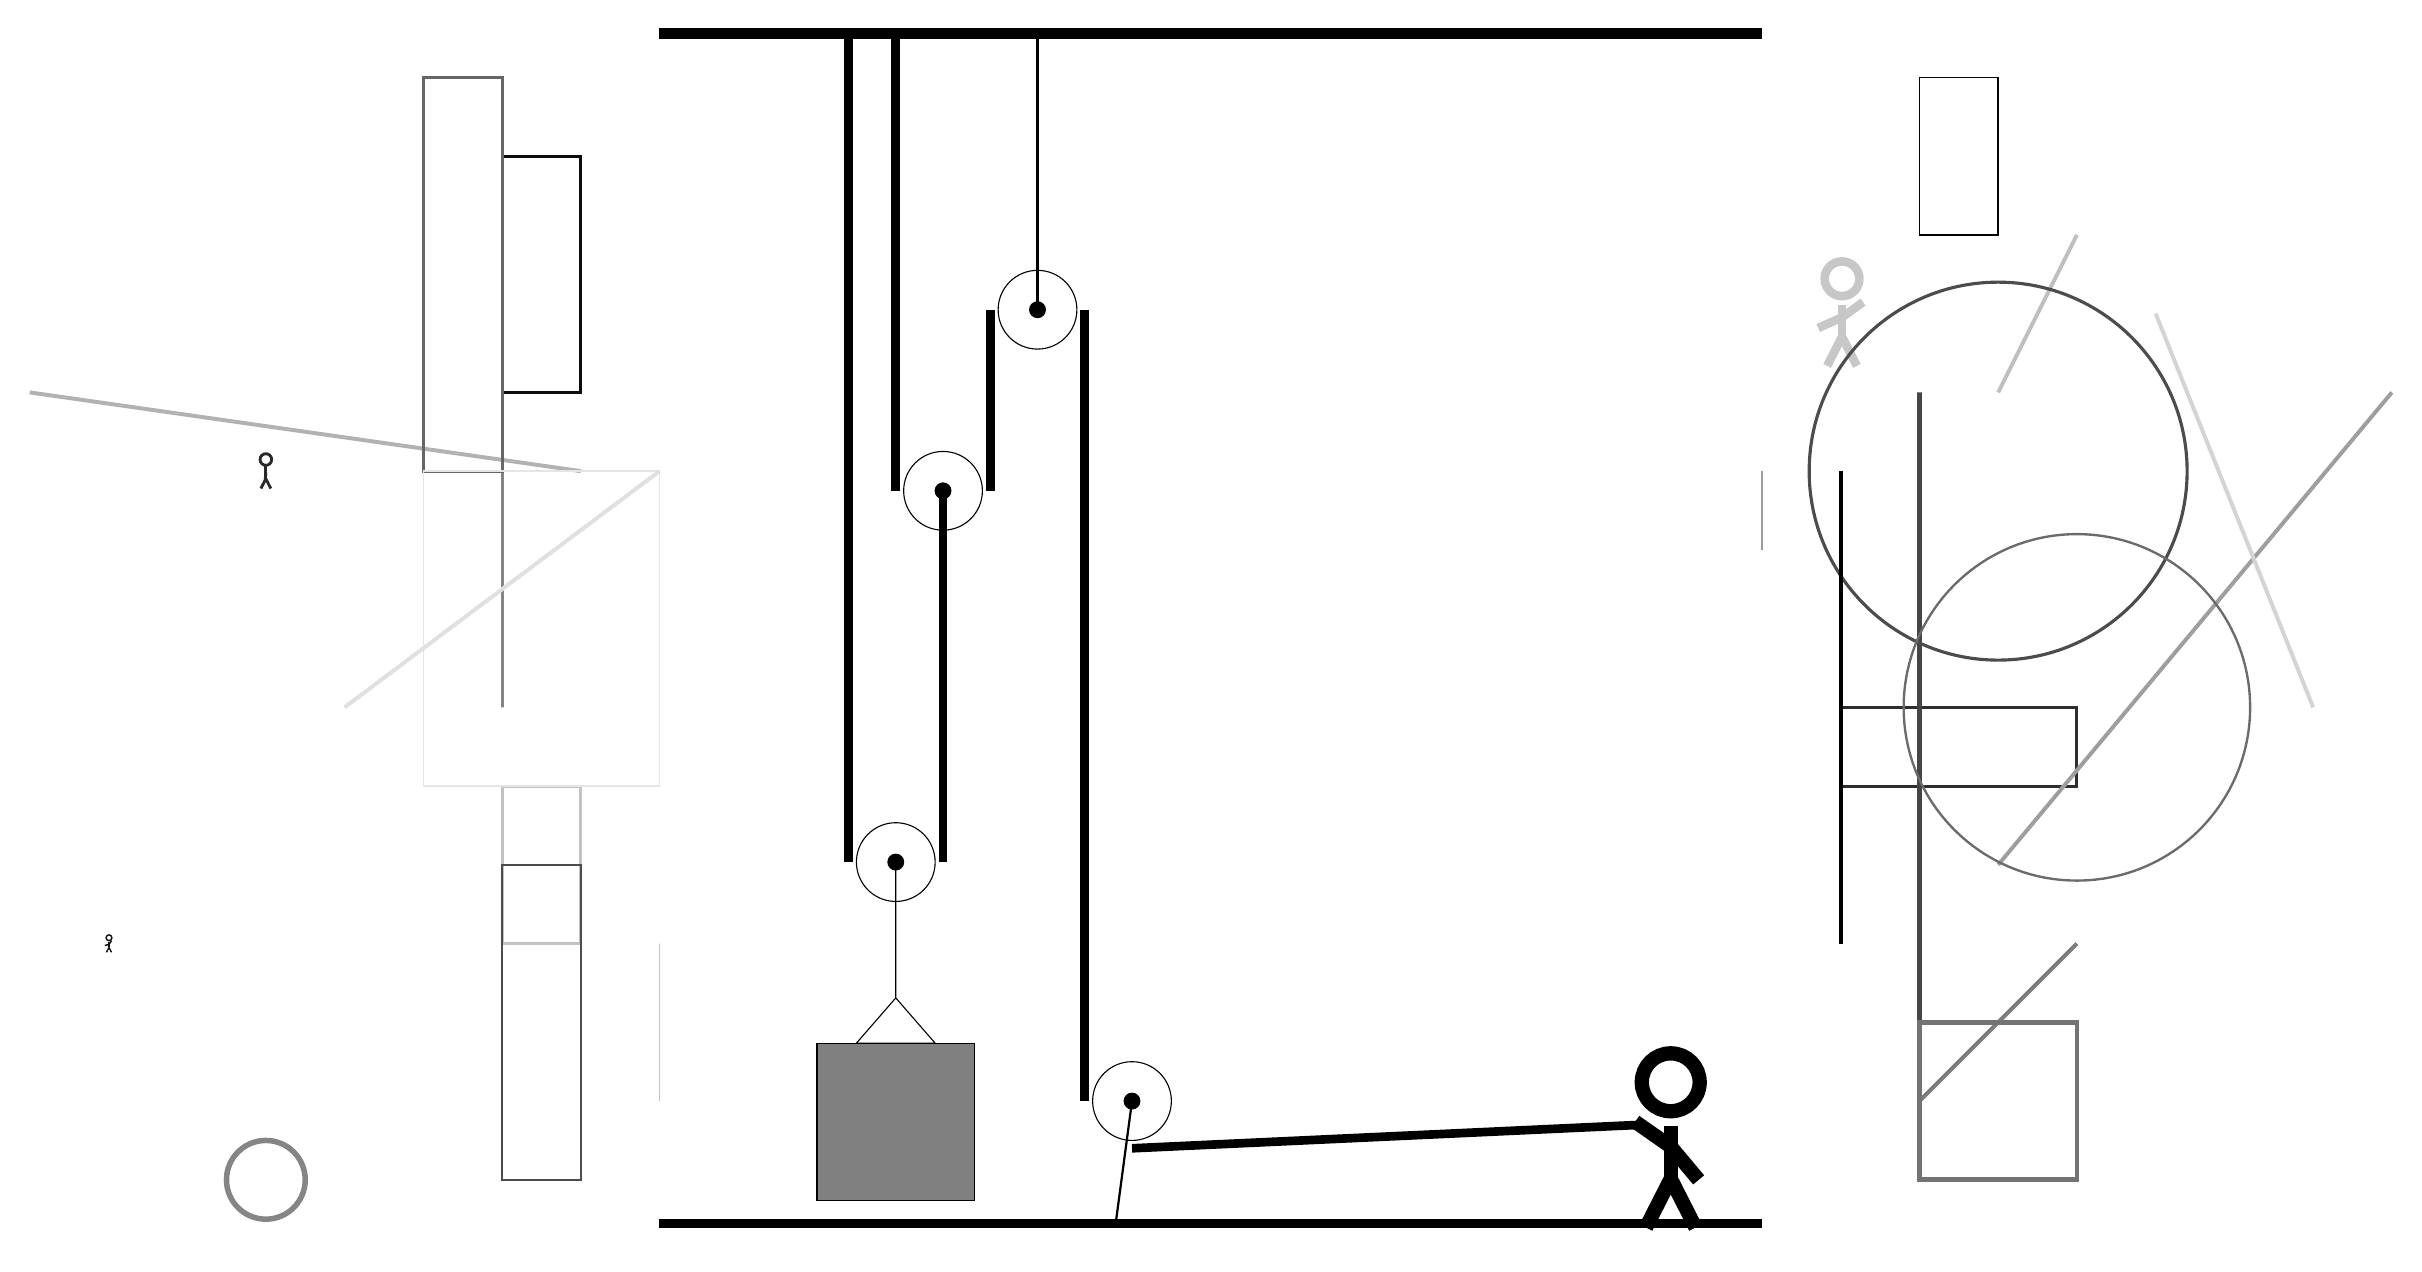
\begin{tikzpicture}
			%%%%% START %%%%%
			
			\draw[fill=black] (-2, 11.5) rectangle (12, 11.625);
			
			\draw (1, 1.035) circle (0.5);
			\draw[fill=black] (1, 1.035) circle (0.1);
			
			\draw (1.6, 5.75) circle (0.5);
			\draw[fill=black] (1.6, 5.75) circle (0.1);
			
			\draw (2.8, 8.05) circle (0.5);
			\draw[fill=black] (2.8, 8.05) circle (0.1);
			\draw[thick] (2.8, 8.05) -- (2.8, 11.5);
			
			\draw (4.0, -2) circle (0.5);
			\draw[fill=black] (4.0, -2) circle (0.1);
			\draw[thick] (4.0, -2) -- (3.8, -3.5);
			
			\draw (1, 1.035) -- (1, -0.69) -- (0.5, -1.265) -- (1.5, -1.265) -- (1, -0.69);
			\draw[fill=black!50] (0, -1.265) rectangle (2, -3.265);
			\draw[line width=1.1mm] (0.4, 11.5) -- (0.4, 1.035);
			\centerarc[line width=1.1mm](1, 1.035)(180:360:0.6);
			\draw[line width=1.1mm](1.6, 1.035) -- (1.6, 5.75);
			\draw[line width=1.1mm] (1.0, 11.5) -- (1.0, 5.75);
			\centerarc[line width=1.1mm](1.6, 5.75)(180:360:0.6);
			\draw[line width=1.1mm](2.2, 5.75) -- (2.2, 8.05);
			\centerarc[line width=1.1mm](2.8, 8.05)(0:180:0.6);
			\draw[line width=1.1mm] (3.4, 8.05) -- (3.4, -2);
			\centerarc[line width=1.1mm](4.0, -2)(0:90:-0.6);
			\draw[line width=1.1mm](4.0, -2.6) -- (10.5, -2.3);
			
			\draw[line width=0.2mm, color=black!24] (-2, 0) rectangle (-2, -2);
			
			\draw[line width=0.4mm, color=black!24] (-3, 2) rectangle (-4, 0);
			\draw[line width=0.5mm, color=black!30](-3, 6) -- (-10, 7);
			\draw[line width=0.3mm, color=black!70] (-4, -3) rectangle (-3, 1);
			\draw[line width=0.4mm, color=black!82] (13, 3) rectangle (16, 2);
			\draw[line width=0.6mm, color=black!73] (14, -2) rectangle (14, 7);
			
			\draw[line width=0.4mm, color=black!48] (-4, 3) rectangle (-4, 7);
			\node[line width=0.6mm, color=black!94] at (-9, 0) {\Strichmaxerl[1][18][53]};
			\node[line width=0.6mm, color=black!22] at (13, 8) {\Strichmaxerl[6][24][36]};
			\node[line width=0.5mm, color=black!84] at (-7, 6) {\Strichmaxerl[2][85][90]};
			
			\draw[line width=0.5mm, color=black!25](15, 7) -- (16, 9);
			\draw[line width=0.4mm, color=black!95] (-3, 7) rectangle (-4, 10);
			\draw[line width=0.5mm, color=black!51](16, 0) -- (14, -2);
			
			\draw[line width=0.4mm, color=black!60] (-4, 11) rectangle (-5, 6);
			\draw [line width=0.5mm, color=black!76](-5, 6) circle (0.0);
			\draw [line width=0.4mm, color=black!70](15, 6) circle (2.4);
			
			\draw[line width=0.2mm, color=black!10] (-2, 6) rectangle (-5, 2);
			
			\draw[line width=0.5mm, color=black!38](15, 1) -- (20, 7);
			\draw[line width=0.3mm, color=black!39] (12, 6) rectangle (12, 5);
			
			\draw[line width=0.2mm, color=black!98] (14, 9) rectangle (15, 11);
			\draw[line width=0.5mm, color=black!12](-6, 3) -- (-2, 6);
			
			\draw [line width=0.7mm, color=black!48](-7, -3) circle (0.5);
			
			\draw[line width=0.5mm, color=black!17](17, 8) -- (19, 3);
			\draw [line width=0.3mm, color=black!58](16, 3) circle (2.2);
			\draw[line width=0.5mm, color=black!100](13, 6) -- (13, 0);
			\draw[line width=0.6mm, color=black!55] (14, -1) rectangle (16, -3);
			
			
			\node at (10.8, -2.5) {\Strichmaxerl[10][-35][-50]};
			
			\draw[fill=black] (-2, -3.5) rectangle (12, -3.6);
			
			%%%%% END %%%%%
		\end{tikzpicture}
	\end{figure}	
\end{document}